\chapter{Interfaces, tensioactifs et colloïdes}\label{ch:b3:colloids}

La mayonnaise est de l'huile dispersée en gouttelettes de quelques
micromètres dans un peu d'eau et de vinaigre, maintenues séparées par la
lécithine et les protéines du jaune d'œuf. Fouettée trop vite au début,
ou avec l'huile versée trop rapidement, elle se sépare en une couche
huileuse et une couche aqueuse~: les gouttelettes fusionnent, et
l'énergie qui les tenait séparées a disparu. Le lait, le brouillard,
l'encre, la peinture, le sang et l'eau boueuse d'une rivière sont de la
même nature~: des particules ou des gouttelettes bien plus grandes que
les molécules et bien plus petites que tout ce que voit l'œil, si
nombreuses que la plupart de leurs molécules sont proches d'une
interface. Ce chapitre traite de l'énergie des interfaces, des molécules
qui l'abaissent, des \omterm{def:b3:colloids:colloid}{colloïdes} que les interfaces rendent possibles, et
de ce qui maintient les \omterm{def:b3:colloids:colloid}{colloïdes} dispersés ou les fait coaguler.

\begin{recall}
Le volume de première année a qualifié d'amphiphile une molécule à tête
hydrophile et à queue hydrophobe, et a décrit les interactions de London
et la permittivité relative des solvants~; le livre 1 (année 11) a
rencontré les \omterm{def:b3:colloids:micelle}{micelles} dans le savon. Le volume de deuxième année a
défini le potentiel chimique, la force ionique et l'activité. Le
\Cref{ch:b3:surfaces-catalysis} a traité de l'\omterm{def:b3:surfaces-catalysis:adsorption}{adsorption} sur les solides,
le \cref{ch:b3:electrode-kinetics} de la \omterm{def:b3:electrode-kinetics:double-layer}{double couche électrique} et de
sa \omterm{def:b3:electrode-kinetics:double-layer}{longueur de Debye}. De la physique~: le mouvement brownien, et la
pression à l'intérieur d'une surface courbe.
\end{recall}

\begin{omfigure}
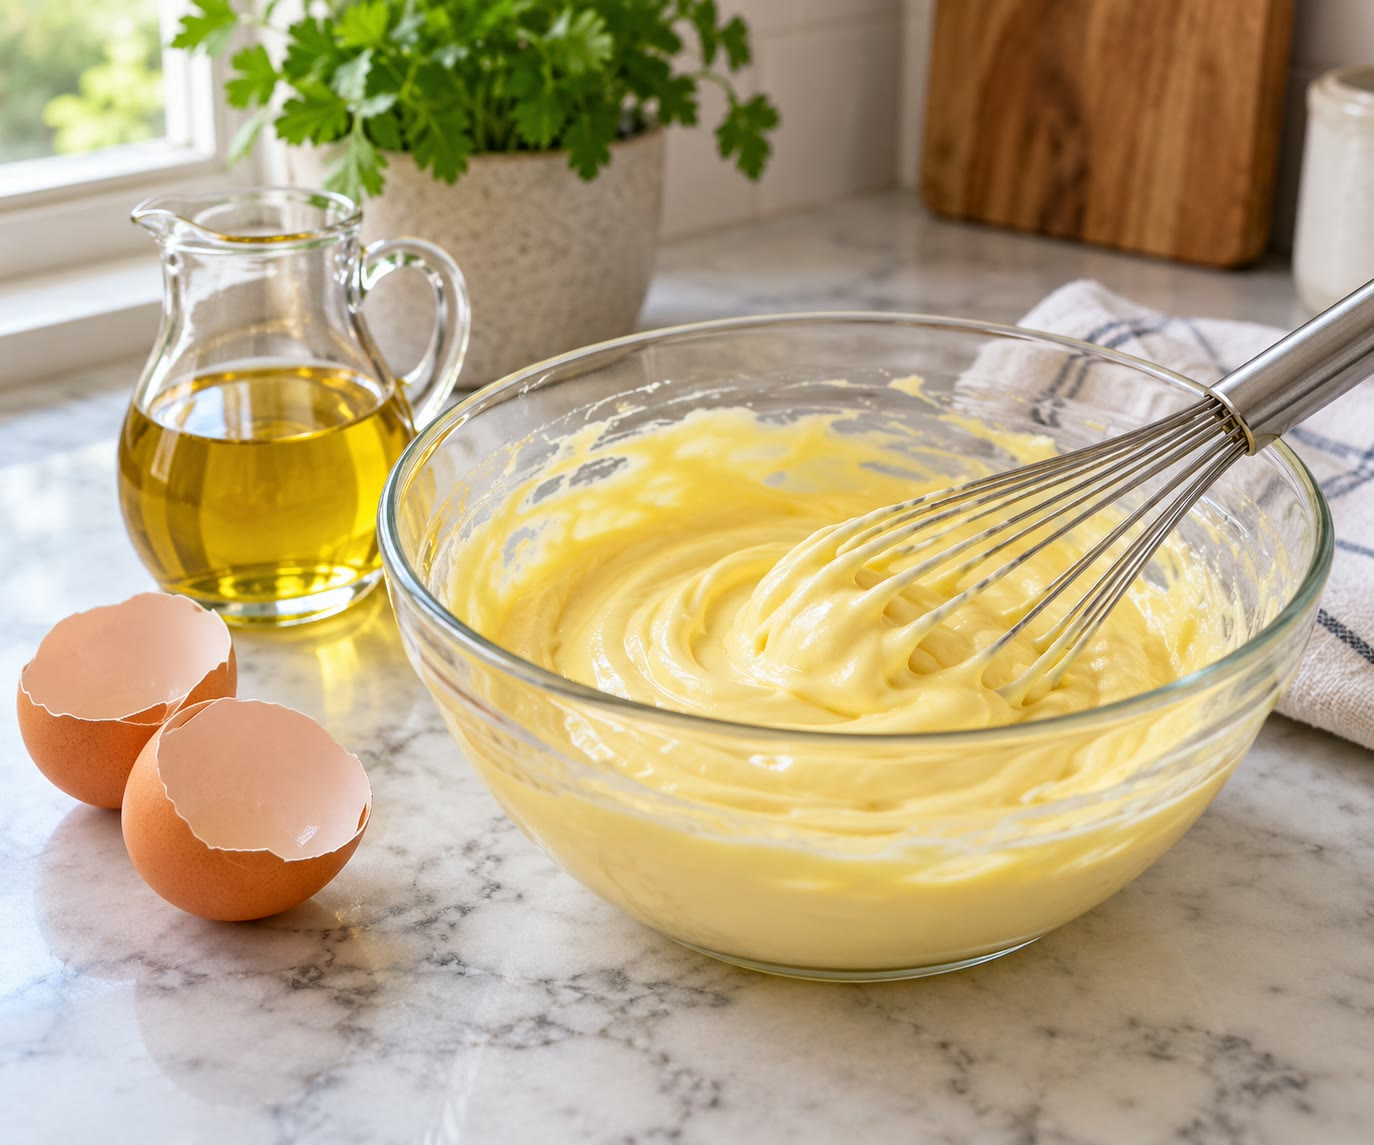
\includegraphics[width=0.6\linewidth]{images/book4/ai/b3-17-mayonnaise.jpg}

{\small Une mayonnaise qu'on fouette~: une \omterm{def:b3:colloids:colloid}{émulsion} de gouttelettes
d'huile dans l'eau, stabilisée par les \omterm{def:b3:colloids:surfactant}{tensioactifs} du jaune d'œuf.}
\end{omfigure}

\section{Interfaces et tension superficielle}

Une molécule au sein d'un liquide est attirée également dans toutes les
directions~; à la surface, elle perd une partie de ses voisines. Créer de
la surface coûte de l'énergie.

\begin{definition}[Tension superficielle]\label{def:b3:colloids:surface-tension}
La \emph{tension superficielle}\index{tension superficielle} $\gamma$ d'un
liquide est l'enthalpie libre nécessaire pour créer une unité d'aire de
sa surface à température, pression et composition constantes~:
$\gamma = (\partial G/\partial A)_{T,p,n}$, en \unit{J.m^{-2}} $=$ \unit{N.m^{-1}}.
Pour une interface entre deux phases, c'est la tension interfaciale.
\end{definition}

L'eau, cohésive grâce aux liaisons hydrogène, a une \omterm{def:b3:colloids:surface-tension}{tension superficielle}
élevée~: \qty{72.0}{mN/m}
à \qty{25}{\celsius}. Les alcanes ont environ 20, le mercure environ 480.

\begin{proposition}[Pression de Laplace]\label{prop:b3:colloids:laplace}
La pression à l'intérieur d'une goutte ou d'une bulle sphérique de rayon
$r$ dépasse la pression extérieure de
\[
  \Delta p = \frac{2\gamma}{r} .
\]
\end{proposition}

\begin{proof}
Augmentons le rayon de $\dd r$ à l'équilibre~: le travail de la
différence de pression, $\Delta p\,4\pi r^2\dd r$, est égal à
l'accroissement de l'enthalpie libre de surface, $\gamma\,8\pi r\,\dd r$.
\end{proof}

\begin{definition}[Angle de contact, mouillage]\label{def:b3:colloids:wetting}
L'\emph{angle de contact}\index{angle de contact} $\theta$ d'une goutte
sur un solide est l'angle, mesuré à travers le liquide, entre la surface
du solide et la surface du liquide sur la ligne où se rencontrent le
solide, le liquide et la vapeur. Un liquide \emph{mouille}\index{mouillage}
le solide quand $\theta < 90^\circ$, et s'étale complètement quand
$\theta = 0$.
\end{definition}

\begin{theorem}[Relation de Young]\label{thm:b3:colloids:young}
À l'équilibre, les trois tensions interfaciales et l'\omterm{def:b3:colloids:wetting}{angle de contact}
vérifient
\[
  \gamma_{\mathrm{SV}} = \gamma_{\mathrm{SL}} + \gamma_{\mathrm{LV}}\cos\theta .
\]
C'est la \emph{relation de Young}\index{relation de Young}.
\end{theorem}

\begin{proof}
Déplaçons la ligne de contact vers l'extérieur de $\dd x$ (par unité de
longueur de ligne)~: une interface solide--vapeur d'aire $\dd x$ est
remplacée par une interface solide--liquide, et l'interface
liquide--vapeur croît de $\dd x\cos\theta$. L'enthalpie libre varie de
$(\gamma_{\mathrm{SL}} - \gamma_{\mathrm{SV}} + \gamma_{\mathrm{LV}}\cos\theta)\dd x$,
quantité nulle à l'équilibre.
\end{proof}

\begin{omfigure}
\begin{tikzpicture}[font=\small, >=Stealth]
  \fill[black!12] (-3.6,-0.5) rectangle (3.6,0);
  \draw[thick] (-3.6,0) -- (3.6,0);
  \node[anchor=north] at (2.6,-0.05) {solide};
  \fill[omWater!60] (-2.0,0) arc[start angle=160, end angle=20, radius=2.13] -- cycle;
  \draw[thick, omDef] (-2.0,0) arc[start angle=160, end angle=20, radius=2.13];
  % circle centre 0.73 below the solid: a cap smaller than a hemisphere, contact angle 90 - 20 = 70 deg;
  % at the right contact point the liquid surface leaves at 110 deg (up and to the left)
  \draw[->, thick, omThm] (2.0,0) -- ++(110:1.3) node[anchor=south] {$\gamma_{\mathrm{LV}}$};
  \draw[->, thick] (2.0,0) -- (3.3,0) node[anchor=south] {$\gamma_{\mathrm{SV}}$};
  \draw[->, thick] (2.0,0) -- (0.7,0) node[anchor=north, yshift=-1pt] {$\gamma_{\mathrm{SL}}$};
  \draw (1.45,0) arc[start angle=180, end angle=110, radius=0.55];
  \node at (1.33,0.42) {$\theta$};
  \node at (0,0.6) {liquide};
  \node at (-2.8,1.4) {vapeur};
\end{tikzpicture}

{\small Une goutte posée et les trois tensions qui tirent sur sa ligne de
contact~: l'équilibre de leurs composantes le long du solide donne la
\omterm{thm:b3:colloids:young}{relation de Young}~; ici $\theta
\approx 70^\circ$, un liquide partiellement mouillant.}
\end{omfigure}

\begin{theorem}[Équation de Kelvin]\label{thm:b3:colloids:kelvin}
La pression de vapeur d'une goutte sphérique de rayon $r$ dépasse celle
du liquide à surface plane, $p^*$~:
\[
  \ln\frac{p}{p^*} = \frac{2\gamma V_{\mathrm m}}{rRT},
\]
où $V_{\mathrm m}$ est le volume molaire du liquide. C'est
l'\emph{équation de Kelvin}\index{equation de Kelvin@équation de Kelvin}.
\end{theorem}

\begin{proof}
Le liquide de la goutte subit la surpression $2\gamma/r$, qui élève son
potentiel chimique de $V_{\mathrm m}\,2\gamma/r$ (avec
$(\partial\mu/\partial p)_T = V_{\mathrm m}$, le liquide étant
incompressible). La vapeur en équilibre avec lui doit voir son potentiel
chimique élevé d'autant~: $RT\ln(p/p^*) = 2\gamma V_{\mathrm m}/r$.
\end{proof}

Pour une gouttelette d'eau de rayon \qty{10}{nm} à \qty{25}{\celsius},
$2\gamma V_{\mathrm m}/rRT = 0.105$~: sa pression de vapeur
dépasse de 11\,\% celle de l'eau à surface plane. Les petites
gouttelettes s'évaporent tandis que les grosses grossissent, et les
nuages ont besoin de noyaux pour se former~; il en va de même pour la
solubilité des petits cristaux.

\begin{definition}[Mûrissement d'Ostwald]\label{def:b3:colloids:ripening}
Le \emph{mûrissement d'Ostwald}\index{murissement d'Ostwald@mûrissement d'Ostwald} est la croissance des
plus grosses particules ou gouttelettes d'une dispersion aux dépens des
plus petites, due à la solubilité ou à la pression de vapeur plus élevée
des petites particules.
\end{definition}

\section{Tensioactifs et micelles}

\begin{definition}[Tensioactif]\label{def:b3:colloids:surfactant}
Un \emph{tensioactif}\index{tensioactif} (agent de surface) est une
molécule amphiphile qui s'adsorbe aux interfaces et abaisse leur
tension. C'est un
\emph{tensioactif anionique}\index{tensioactif anionique} si sa tête est
un anion (dodécylsulfate de sodium, savons), un \emph{tensioactif
cationique}\index{tensioactif cationique}
si c'est un cation (sels d'ammonium quaternaire), un \emph{tensioactif
non ionique}\index{tensioactif non ionique} si la tête est un groupe
polaire neutre (une chaîne de motifs oxyde d'éthylène).
\end{definition}

\begin{definition}[Concentration superficielle d'excès]\label{def:b3:colloids:surface-excess}
La \emph{concentration superficielle d'excès}\index{concentration superficielle d'exces@concentration superficielle d'excès} $\Gamma$ d'un
soluté est la quantité de soluté à l'interface par unité d'aire, en
excès par rapport à ce que contiendrait le même volume si la
concentration du sein de la solution se maintenait jusqu'à l'interface.
\end{definition}

\begin{theorem}[Isotherme d'adsorption de Gibbs]\label{thm:b3:colloids:gibbs-adsorption}
Pour une solution diluée d'un soluté non ionique de concentration $c$,
\[
  \Gamma = -\frac{1}{RT}\frac{\dd\gamma}{\dd\ln c};
\]
pour un \omterm{def:b3:colloids:surfactant}{tensioactif} ionique 1:1 sans sel ajouté, $RT$ est remplacé par
$2RT$. C'est
l'\emph{isotherme d'adsorption de Gibbs}\index{isotherme d'adsorption de Gibbs}.
\end{theorem}

\begin{proof}
Pour l'interface, l'analogue de la relation de Gibbs--Duhem à $T$ et
$p$ constants s'écrit $\dd\gamma = -\sum_i\Gamma_i\,\dd\mu_i$ (l'enthalpie
libre de surface $\gamma A$ jouant le rôle de $G$,
ce qui est admis). En choisissant la surface de séparation de sorte que
le solvant n'ait pas d'excès,
$\dd\gamma = -\Gamma\,\dd\mu$, et en solution diluée $\dd\mu = RT\,\dd\ln c$.
Pour un \omterm{def:b3:colloids:surfactant}{tensioactif} ionique,
le cation et l'anion sont tous deux adsorbés avec le même excès, et
$\dd\mu$ devient
$2RT\,\dd\ln c$.
\end{proof}

Un \omterm{def:b3:colloids:surfactant}{tensioactif} dont la \omterm{def:b3:colloids:surface-tension}{tension superficielle} décroît linéairement avec
$\ln c$ a un excès superficiel constant~: l'interface est saturée, et
$1/(\Gamma N_A)$ est l'aire occupée par
une molécule adsorbée.

\begin{method}[Aire par molécule à partir d'une pente $\gamma$--$\ln c$]\label{met:b3:colloids:surface-excess}
\begin{enumerate}
  \item Mesurer $\gamma$ en fonction de $c$ au-dessous de la CMC~; tracer
        $\gamma$ en fonction de $\ln c$.
  \item Prendre la pente de la partie linéaire juste au-dessous de la
        CMC~; $\Gamma = -\text{pente}/(nRT)$, $n
        = 1$ pour un \omterm{def:b3:colloids:surfactant}{tensioactif non ionique}, 2 pour un \omterm{def:b3:colloids:surfactant}{tensioactif}
        ionique 1:1 sans sel.
  \item Aire par molécule $= 1/(\Gamma N_A)$~; les valeurs typiques vont
        de 0.3 à \qty{0.6}{nm^2}.
\end{enumerate}
\end{method}

\begin{definition}[Micelle, concentration micellaire critique, nombre d'agrégation]\label{def:b3:colloids:micelle}
Une \emph{micelle}\index{micelle} est un agrégat de molécules de
\omterm{def:b3:colloids:surfactant}{tensioactif} en solution dont les queues hydrophobes forment un cœur
d'aspect liquide, protégé de l'eau par les têtes. La
\emph{concentration micellaire critique}\index{concentration micellaire critique}
(CMC) est la concentration au-delà de laquelle des micelles se forment~;
leur nombre moyen de molécules est le \emph{nombre
d'agrégation}\index{nombre d'agregation@nombre d'agrégation}.
\end{definition}

\begin{proposition}[Ruptures de pente à la CMC]\label{prop:b3:colloids:cmc-break}
Au-delà de la CMC, la concentration en \omterm{def:b3:colloids:surfactant}{tensioactif} libre, et avec elle
la \omterm{def:b3:colloids:surface-tension}{tension superficielle} et la pression osmotique, restent presque
constantes~; les propriétés qui dépendent des molécules libres changent
de pente à la CMC.
\end{proposition}

\begin{proof}[Démonstration partielle]
Traitons les \omterm{def:b3:colloids:micelle}{micelles} comme une phase distincte~: le \omterm{def:b3:colloids:surfactant}{tensioactif} ajouté
passe dans les \omterm{def:b3:colloids:micelle}{micelles} dès que le potentiel chimique des molécules
libres atteint celui d'une molécule dans une \omterm{def:b3:colloids:micelle}{micelle}, et ce potentiel
chimique, donc la concentration libre, reste alors fixé. La \omterm{def:b3:colloids:surface-tension}{tension
superficielle}, fixée par les molécules libres via l'isotherme de Gibbs,
cesse de diminuer~; la conductivité continue d'augmenter, mais plus
lentement, puisque les \omterm{def:b3:colloids:micelle}{micelles} portent moins de charge par molécule de
\omterm{def:b3:colloids:surfactant}{tensioactif} que les ions libres (une partie de leurs contre-ions est
liée). Le modèle est une limite, car les \omterm{def:b3:colloids:micelle}{micelles} de taille finie se
forment sur un étroit domaine de concentration (admis).
\end{proof}

\begin{method}[La CMC par une rupture de pente]\label{met:b3:colloids:cmc}
\begin{enumerate}
  \item Mesurer la \omterm{def:b3:colloids:surface-tension}{tension superficielle} (ou, pour un \omterm{def:b3:colloids:surfactant}{tensioactif}
        ionique, la conductivité) sur un domaine de concentrations qui
        encadre la CMC attendue.
  \item Ajuster des droites sur les deux branches ($\gamma$ en fonction de
        $\log c$, ou $\kappa$ en fonction de $c$).
  \item Leur intersection est la CMC.
\end{enumerate}
\end{method}

\begin{omfigure}
\begin{tikzpicture}
\begin{axis}[name=gm, width=0.47\linewidth, height=5.2cm, xmin=-5, xmax=-1.5, ymin=30, ymax=76,
  axis lines=left, xlabel={$\log(c/\unit{mol.L^{-1}})$}, ylabel={$\gamma$ / \unit{mN.m^{-1}}},
  tick label style={font=\small}, label style={font=\small}]
\addplot[omDef, very thick] table[x=logc, y=gamma_mN] {figdata/out/bachelor-3-surfactant-cmc-gamma.dat};
\draw[black!40, dashed] (axis cs:-2.086,30) -- (axis cs:-2.086,70);
\node[font=\scriptsize, anchor=south west] at (axis cs:-2.05,45) {CMC};
\end{axis}
\begin{axis}[at={(gm.east)}, anchor=west, xshift=1.4cm, width=0.47\linewidth, height=5.2cm,
  xmin=0, xmax=20, ymin=0, ymax=1.0, axis lines=left, xlabel={$c$ / mM},
  ylabel={$\kappa$ / \unit{mS.cm^{-1}}}, tick label style={font=\small}, label style={font=\small}]
\addplot[omThm, very thick] table[x=c_mM, y=kappa] {figdata/out/bachelor-3-surfactant-cmc-kappa.dat};
\draw[black!40, dashed] (axis cs:8.2,0) -- (axis cs:8.2,0.9);
\node[font=\scriptsize, anchor=south west] at (axis cs:8.4,0.15) {CMC};
\end{axis}
\end{tikzpicture}

{\small Un \omterm{def:b3:colloids:surfactant}{tensioactif} ionique modèle ayant la CMC du dodécylsulfate de
sodium,
\qty{8.2}{mM} à \qty{25}{\celsius}. À gauche~: la \omterm{def:b3:colloids:surface-tension}{tension superficielle}
décroît avec $\log c$, linéairement juste au-dessous de la CMC (interface
saturée, environ \qty{0.6}{nm^2} par molécule), puis reste constante.
À droite~: la conductivité croît moins vite au-delà de la CMC.}
\end{omfigure}

\begin{definition}[Paramètre d'empilement]\label{def:b3:colloids:packing}
Le \emph{paramètre d'empilement}\index{parametre d'empilement@paramètre d'empilement} d'un \omterm{def:b3:colloids:surfactant}{tensioactif} vaut $P =
v/(a_0l)$, où $v$ est le volume de sa queue hydrophobe, $l$ la longueur
de la queue étendue et $a_0$ l'aire optimale par tête à la surface de
l'agrégat.
\end{definition}

\begin{proposition}[Forme des agrégats]\label{prop:b3:colloids:packing}
Les \omterm{def:b3:colloids:micelle}{micelles} sphériques exigent $P \le \frac13$, les \omterm{def:b3:colloids:micelle}{micelles}
cylindriques $\frac13 < P \le \frac12$, les bicouches planes
(vésicules, membranes) $\frac12 < P \le 1$~; $P > 1$ donne des structures
inverses.
\end{proposition}

\begin{proof}
Dans une sphère de rayon $R \le l$ formée de $N$ molécules, $Nv = \frac43\pi R^3$ et $Na_0 = 4\pi R^2$, donc
$v/a_0 = R/3 \le l/3$~: $P \le \frac13$. Pour un cylindre de rayon $R$ et
de longueur $L$, $Nv = \pi R^2L$ et
$Na_0 = 2\pi RL$~: $v/a_0 = R/2 \le l/2$. Pour une bicouche d'épaisseur
$2l$ et d'aire $A$, $Nv = 2lA$ et
$Na_0 = 2A$~: $v/a_0 = l$.
\end{proof}

\begin{omfigure}
\begin{tikzpicture}[font=\scriptsize]
  % a sphere-forming cone
  \draw[omDef, thick, fill=omDef!15] (0,0) -- (-0.45,1.2) arc[start angle=180, end angle=0, radius=0.45] -- cycle;
  \node at (0,-0.3) {$P < \frac13$~: cône};
  % micelle
  \begin{scope}[xshift=2.2cm, yshift=0.6cm]
    \foreach \a in {0,30,...,330}{\draw[black!60] (\a:0.2) -- (\a:0.62); \fill[omDef] (\a:0.7) circle (0.09);}
    \node at (0,-1.05) {micelle sphérique};
  \end{scope}
  % truncated cone
  \begin{scope}[xshift=4.7cm]
    \draw[omDef, thick, fill=omDef!15] (-0.18,0) -- (-0.4,1.2) -- (0.4,1.2) -- (0.18,0) -- cycle;
    \node at (0,-0.3) {$\frac13 < P < \frac12$};
  \end{scope}
  \begin{scope}[xshift=6.9cm, yshift=0.6cm]
    \fill[omDef!10] (-0.9,-0.55) rectangle (0.9,0.55);
    \foreach \x in {-0.8,-0.5,...,0.8}{\fill[omDef] (\x,0.62) circle (0.08); \fill[omDef] (\x,-0.62) circle (0.08);}
    \node at (0,-1.05) {cylindre (de profil)};
  \end{scope}
  % cylinder shape
  \begin{scope}[xshift=9.4cm]
    \draw[omDef, thick, fill=omDef!15] (-0.3,0) rectangle (0.3,1.2);
    \node at (0,-0.3) {$P \approx 1$~: cylindre};
  \end{scope}
  \begin{scope}[xshift=11.4cm, yshift=0.6cm]
    \foreach \x in {-0.8,-0.6,...,0.8}{
      \draw[black!60] (\x,0.5) -- (\x,0.05) (\x,-0.5) -- (\x,-0.05);
      \fill[omDef] (\x,0.58) circle (0.08); \fill[omDef] (\x,-0.58) circle (0.08);}
    \node at (0,-1.05) {bicouche};
  \end{scope}
\end{tikzpicture}

{\small Forme moléculaire et forme de l'agrégat. Un \omterm{def:b3:colloids:surfactant}{tensioactif} à grosse
tête et à queue unique (un cône) s'assemble en \omterm{def:b3:colloids:micelle}{micelles} sphériques~; à
tête plus petite, en cylindres~; une molécule aussi large à la queue qu'à
la tête, comme un lipide à deux chaînes, en bicouches planes, parois des
vésicules et membranes cellulaires.}
\end{omfigure}

La détergence combine ces effets~: le \omterm{def:b3:colloids:surfactant}{tensioactif} abaisse la tension
interfaciale entre l'eau et une salissure grasse jusqu'à ce que la
salissure se roule en gouttes, que les \omterm{def:b3:colloids:micelle}{micelles} solubilisent ensuite
dans leur cœur.

\section{Les colloïdes}

\begin{definition}[Colloïde]\label{def:b3:colloids:colloid}
Un \emph{colloïde}\index{colloide@colloïde} est une dispersion de
particules, de gouttelettes ou de bulles,
d'une taille allant d'environ \qty{1}{nm} à \qty{1}{\micro m} (la
\emph{phase dispersée}\index{phase dispersee@phase dispersée}), dans un
\emph{milieu dispersant}\index{milieu dispersant} continu. Un
\emph{sol}\index{sol} est une dispersion de particules solides dans un
liquide, une \emph{émulsion}\index{emulsion@émulsion} une dispersion de
gouttelettes liquides dans un autre liquide, une
\emph{mousse}\index{mousse} une dispersion de bulles de gaz dans un
liquide ou un solide, un \emph{gel}\index{gel}
un réseau de particules ou de polymères qui occupe tout le liquide et lui
donne la consistance d'un solide, un \emph{aérosol}\index{aerosol@aérosol}
une dispersion de gouttelettes ou de particules dans un gaz.
\end{definition}

Les particules colloïdales sont assez petites pour rester en suspension
grâce au mouvement brownien (les chocs aléatoires des molécules de
solvant, vus en physique) et assez grandes pour diffuser la lumière.

\begin{definition}[Effet Tyndall]\label{def:b3:colloids:tyndall}
L'\emph{effet Tyndall}\index{effet Tyndall} est la diffusion de la lumière
par les particules d'un \omterm{def:b3:colloids:colloid}{colloïde}, qui rend un faisceau visible de côté
quand il traverse le \omterm{def:b3:colloids:colloid}{colloïde}, alors qu'une vraie solution reste
invisible.
\end{definition}

\begin{omfigure}
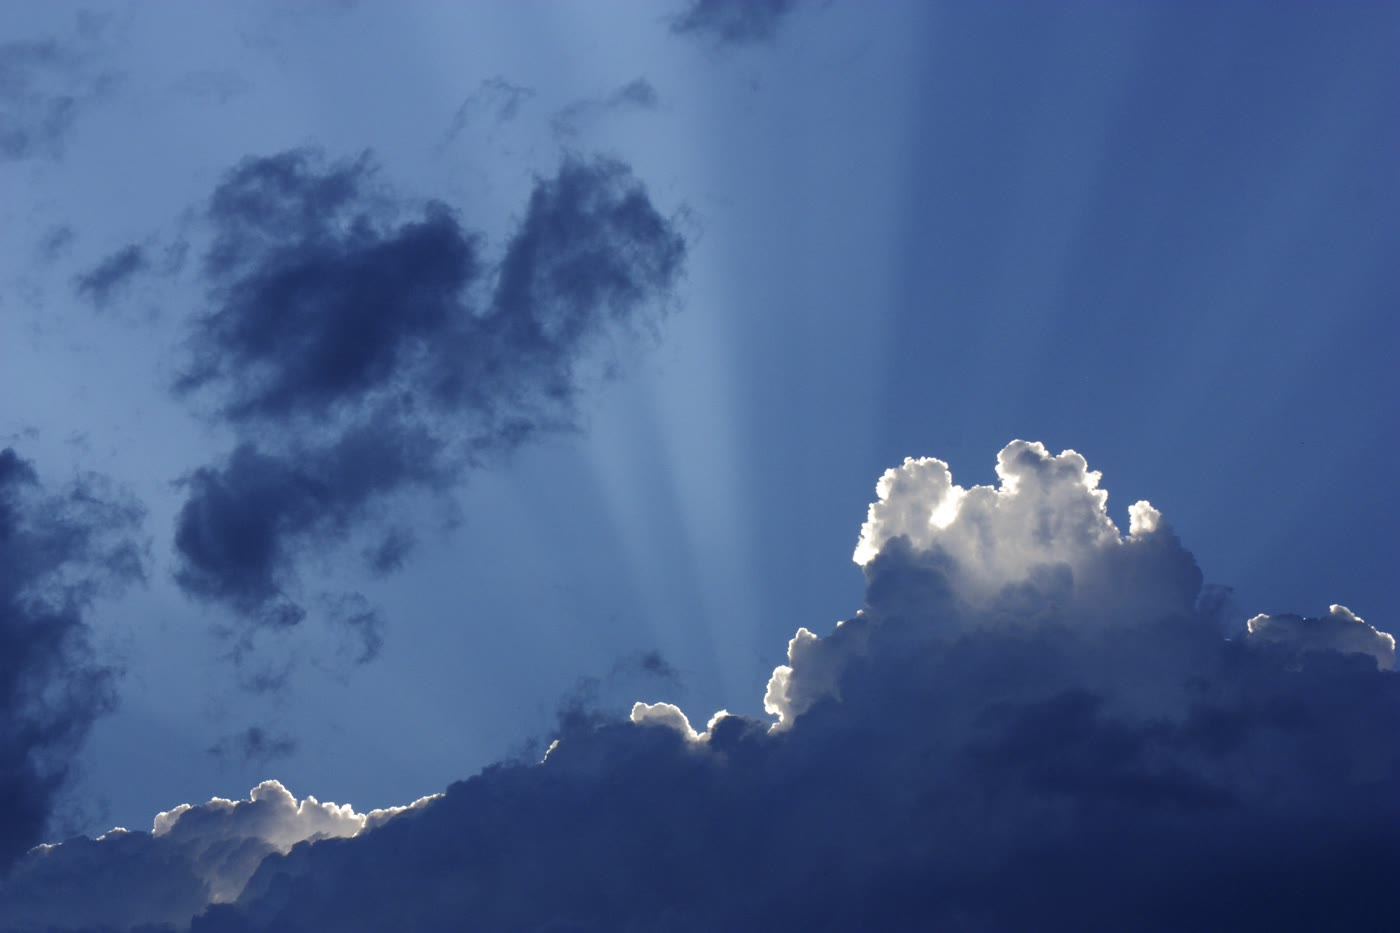
\includegraphics[width=0.55\linewidth]{images/book4/tyndall-sky.jpg}

{\small Rayons de soleil passant par une trouée dans les nuages~: ils sont
visibles parce que l'\omterm{def:b3:colloids:colloid}{aérosol} de l'air, gouttelettes et poussières,
diffuse latéralement une partie de la lumière, l'\omterm{def:b3:colloids:tyndall}{effet Tyndall} à
l'échelle du ciel.}
\end{omfigure}

\section{La stabilité colloïdale}

Deux particules colloïdales s'attirent toujours à courte portée par les
forces de van der Waals. Dans l'eau, la plupart des particules portent
aussi une charge (groupes de surface ionisés, ions adsorbés), entourée
d'une \omterm{def:b3:electrode-kinetics:double-layer}{couche diffuse} de contre-ions, la double couche du
\cref{ch:b3:electrode-kinetics}. Quand deux particules s'approchent,
leurs \omterm{def:b3:electrode-kinetics:double-layer}{couches diffuses} se recouvrent et se repoussent.

\begin{definition}[Potentiel zêta]\label{def:b3:colloids:zeta}
Le \emph{potentiel zêta}\index{potentiel zeta@potentiel zêta} $\zeta$ d'une particule est le
potentiel électrique à son plan de cisaillement, la frontière, au sein
de la double couche, entre le liquide qui se déplace avec la particule
et celui qui ne le fait pas~; on le mesure à partir de la vitesse des
particules dans un champ électrique
(électrophorèse).
\end{definition}

\begin{omfigure}
\begin{tikzpicture}[font=\scriptsize]
  \fill[black!20] (0,0) circle (1.2);
  \foreach \a in {0,30,...,330}{\node at (\a:1.05) {$-$};}
  \draw[omDef, dashed] (0,0) circle (1.55);
  \foreach \a in {15,45,...,345}{\draw[omDef, fill=omDef!15] (\a:1.38) circle (0.11); \node at (\a:1.38) {\tiny$+$};}
  \draw[omThm, thick, densely dotted] (0,0) circle (1.85);
  \foreach \a/\r/\s in {10/2.2/+, 50/2.5/+, 95/2.3/-, 130/2.7/+, 175/2.2/+, 215/2.6/-, 250/2.3/+, 290/2.8/+, 345/2.6/+}{
    \draw[black!60, fill=white] (\a:\r) circle (0.11); \node at (\a:\r) {\tiny$\s$};}
  \draw[->, black!60] (2.6,1.6) node[anchor=west] {couche de Stern} -- (40:1.6);
  \draw[->, omThm] (2.6,-1.4) node[anchor=west] {plan de cisaillement~: $\zeta$} -- (-30:1.87);
  \node at (0,0) {particule};
  \node[anchor=west] at (2.9,0.2) {couche diffuse};
\end{tikzpicture}

{\small Une particule chargée négativement avec sa double couche~: une
couche compacte de Stern, formée de contre-ions, le plan de cisaillement
juste au-delà, où est défini le \omterm{def:b3:colloids:zeta}{potentiel zêta}, et la \omterm{def:b3:electrode-kinetics:double-layer}{couche diffuse},
dans laquelle les contre-ions sont plus nombreux que les co-ions sur
quelques \omterm{def:b3:electrode-kinetics:double-layer}{longueurs de Debye}.}
\end{omfigure}

\begin{theorem}[Théorie DLVO]\label{thm:b3:colloids:dlvo}
Pour deux sphères de rayon $a$ séparées d'un intervalle $h \ll a$, de
potentiel de \omterm{def:b3:electrode-kinetics:double-layer}{couche diffuse}
$\psi$ et de constante de Hamaker $A$, l'énergie d'interaction vaut, aux
faibles potentiels,
\[
  V(h) = 2\pi\varepsilon_r\varepsilon_0a\psi^2\ln\bigl(1 + \eu^{-\kappa h}\bigr) - \frac{Aa}{12h} .
\]
Le premier terme, la répulsion de double couche, décroît sur la \omterm{def:b3:electrode-kinetics:double-layer}{longueur
de Debye} $\kappa^{-1}$~;
le second, l'attraction de van der Waals, ne dépend pas du sel. Leur
somme présente une barrière d'énergie à quelques \omterm{def:b3:electrode-kinetics:double-layer}{longueurs de Debye}
quand la concentration en sel est faible, et aucune au-delà d'une
concentration critique.
\end{theorem}

\begin{proof}[Démonstration partielle]
Les deux formes sont admises (la répulsion à partir du recouvrement de
deux couches de Gouy--Chapman dans l'approximation de Derjaguin,
l'attraction en sommant les interactions de London sur les deux corps).
Augmenter la force ionique augmente $\kappa$
(\cref{prop:b3:electrode-kinetics:debye-length})~: la répulsion
s'éteint alors à plus petite distance $h$, là où l'attraction, qui croît
comme $1/h$, est plus forte~; le maximum
de $V$ diminue et finit par disparaître.
\end{proof}

\begin{omfigure}
\begin{tikzpicture}
\begin{axis}[width=0.72\linewidth, height=5.6cm, xmin=0, xmax=30, ymin=-40, ymax=45,
  axis lines=left, xlabel={intervalle $h$ / nm}, ylabel={$V/kT$},
  tick label style={font=\small}, label style={font=\small},
  legend style={font=\scriptsize, draw=none, at={(0.98,0.98)}, anchor=north east}, legend cell align=left]
\addplot[omDef, thick] table[x=h_nm, y=I1] {figdata/out/bachelor-3-dlvo.dat};
\addplot[black!60, thick] table[x=h_nm, y=I10] {figdata/out/bachelor-3-dlvo.dat};
\addplot[omThm, thick] table[x=h_nm, y=I50] {figdata/out/bachelor-3-dlvo.dat};
\addplot[black, thick, dashed] table[x=h_nm, y=I200] {figdata/out/bachelor-3-dlvo.dat};
\draw[black!30] (axis cs:0,0) -- (axis cs:30,0);
\legend{\qty{1}{mM}, \qty{10}{mM}, \qty{50}{mM}, \qty{200}{mM}}
\end{axis}
\end{tikzpicture}

{\small Interaction DLVO de deux particules de rayon \qty{100}{nm}
(modèle~: potentiel de \omterm{def:b3:electrode-kinetics:double-layer}{couche diffuse}
\qty{-30}{mV}, constante de Hamaker \qty{2e-20}{J}) dans l'eau contenant
un sel 1:1. À \qty{1}{mM}, une barrière d'environ $40\,kT$ maintient les
particules séparées~; à \qty{10}{mM}, elle est réduite de moitié~;
vers \qty{50}{mM}, elle disparaît et toute collision est collante.}
\end{omfigure}

\begin{definition}[Coagulation et stabilisation]\label{def:b3:colloids:stability}
La \emph{coagulation}\index{coagulation} est l'agrégation de particules
colloïdales due à la perte de leur répulsion électrostatique~; la
\emph{floculation}\index{floculation}
est une agrégation en flocs lâches, souvent pontés par des polymères
adsorbés. La
\emph{concentration critique de coagulation}\index{concentration critique de coagulation}
(CCC) d'un électrolyte est la concentration au-delà de laquelle un
\omterm{def:b3:colloids:colloid}{colloïde} coagule rapidement. La \emph{stabilisation stérique}\index{stabilisation sterique@stabilisation stérique}
maintient les particules séparées par des chaînes de polymère adsorbées
ou greffées, dont le recouvrement coûterait de l'entropie.
\end{definition}

\begin{proposition}[Règle de Schulze--Hardy]\label{prop:b3:colloids:schulze-hardy}
Pour un \omterm{def:b3:colloids:colloid}{colloïde} fortement chargé, la \omterm{def:b3:colloids:stability}{concentration critique de
coagulation} d'un électrolyte varie comme l'inverse de la puissance six
de la charge $z$ de ses contre-ions~: $\text{CCC} \propto z^{-6}$, dans
les rapports $1 : \frac{1}{64} : \frac{1}{729}$ pour $z = 1, 2, 3$.
\end{proposition}

\begin{proof}[Démonstration partielle]
Traitons deux plaques planes. À potentiel de surface élevé, la répulsion
de double couche par unité d'aire tend vers $V_R = (64nkT/\kappa)\eu^{-\kappa h}$,
où $n$ est la densité en nombre de l'électrolyte $z{:}z$,
indépendamment du potentiel (admis)~; l'attraction vaut $V_A =
-A/(12\pi h^2)$. À la CCC, la barrière s'annule tout juste~: $V = 0$ et
$\dd V/\dd h = 0$ pour le même
intervalle. Comme $\dd V_R/\dd h = -\kappa V_R$ et $\dd V_A/\dd h = -2V_A/h$,
les deux conditions donnent
$\kappa V_R = 2V_R/h$, donc $\kappa h = 2$, puis $64nkT\eu^{-2}/\kappa = A\kappa^2/(48\pi)$, c'est-à-dire $n \propto \kappa^3$. Avec
$\kappa^2 = 2nz^2e^2/(\varepsilon kT)$, $\kappa^3 \propto (nz^2)^{3/2}$ et $n \propto n^{3/2}z^3$~: donc $n \propto z^{-6}$.
\end{proof}

\begin{omfigure}
\begin{tikzpicture}[font=\small, >=Stealth]
  \foreach \x/\lab/\v in {0/\ce{Na+}/1, 2.6/\ce{Ca^{2+}}/{1/64}, 5.2/\ce{Al^{3+}}/{1/729}}{
    \node at (\x,0) {\lab};
    \node[font=\scriptsize] at (\x,-0.45) {CCC $\times\,\v$};}
  \draw[->, thick, omDef] (-0.8,-0.95) -- (6.0,-0.95) node[midway, below, font=\scriptsize] {dose plus faible pour coaguler un colloïde négatif};
\end{tikzpicture}

{\small La règle de Schulze--Hardy pour un \omterm{def:b3:colloids:colloid}{colloïde} chargé négativement~:
la \omterm{def:b3:colloids:stability}{concentration critique de coagulation} décroît comme la puissance six
de la charge du contre-ion.}
\end{omfigure}

Cette règle explique pourquoi les sels d'aluminium sont si efficaces pour
clarifier l'eau, et pourquoi les fleuves déposent leur charge d'argile là
où ils rencontrent l'eau salée de la mer.

\begin{method}[Choisir une dose de coagulant]\label{met:b3:colloids:coagulant-dose}
\begin{enumerate}
  \item Mesurer la CCC d'un électrolyte de référence pour la suspension
        (essais de \omterm{def:b3:colloids:stability}{floculation} en bécher à doses croissantes, en
        observant la décantation).
  \item La transposer au contre-ion du coagulant avec la règle de
        Schulze--Hardy.
  \item Convertir en masse de sel par mètre cube à l'aide de sa formule~;
        en ajouter assez pour l'hydrolyse et pour l'alcalinité qu'elle
        consomme.
  \item Éviter le surdosage~: des contre-ions fortement chargés peuvent
        inverser le signe de la charge des particules et les restabiliser.
\end{enumerate}
\end{method}

\section{Les colloïdes à l'œuvre}

\begin{definition}[Balance hydrophile--lipophile]\label{def:b3:colloids:hlb}
La \emph{balance hydrophile--lipophile}\index{balance hydrophile--lipophile}
(HLB) d'un \omterm{def:b3:colloids:surfactant}{tensioactif non ionique} vaut, dans l'échelle de Griffin, $20$
fois la fraction massique de sa partie hydrophile~: les faibles valeurs
(3 à 6) conviennent aux \omterm{def:b3:colloids:colloid}{émulsions} eau dans huile, les valeurs élevées
(8 à 18) aux \omterm{def:b3:colloids:colloid}{émulsions} huile dans eau et aux détergents.
\end{definition}

Les \omterm{def:b3:colloids:colloid}{émulsions} sont thermodynamiquement instables, puisque chaque
gouttelette porte une énergie interfaciale~; les émulsifiants les
rendent cinétiquement stables en abaissant cette énergie et en ajoutant
une couche répulsive, chargée ou stérique, autour de chaque gouttelette.
La mayonnaise est une \omterm{def:b3:colloids:colloid}{émulsion} huile dans eau si riche en huile (environ
les quatre cinquièmes du volume) que les gouttelettes sont comprimées
les unes contre les autres, ce qui en fait un solide mou. Les \omterm{def:b3:colloids:colloid}{mousses}
sont stabilisées par des \omterm{def:b3:colloids:surfactant}{tensioactifs} qui ralentissent l'écoulement du
liquide dans les films séparant les bulles~; les antimousses, souvent des
huiles silicones, s'étalent sur ces films et les rompent. Dans les usines
de potabilisation, les sels d'aluminium ou de fer(III) coagulent les
\omterm{def:b3:colloids:colloid}{colloïdes} argileux et organiques qui troublent l'eau des rivières~;
l'hydroxyde qu'ils forment entraîne les flocs vers le fond en
sédimentant. Les nanoparticules métalliques sont maintenues dispersées
par des ions citrate adsorbés (stabilisation électrostatique) ou par des
chaînes de polymère liées par des thiols (\omterm{def:b3:colloids:stability}{stabilisation stérique}).

\begin{inthelab}[L'anneau de du Noüy]
Un anneau de platine, passé à la flamme pour le nettoyer, est suspendu à
une balance et plongé horizontalement dans le liquide, puis remonté
lentement. La force nécessaire pour l'arracher à la surface passe par un
maximum~; divisée par le double de la circonférence de l'anneau et
corrigée de la forme du ménisque soulevé, elle donne la \omterm{def:b3:colloids:surface-tension}{tension
superficielle}. La mesure d'une série de \omterm{def:b3:colloids:surfactant}{tensioactifs} commence par la
solution la plus diluée, en rinçant l'anneau entre deux échantillons.
\end{inthelab}

\begin{safety}{\ghs[0.8cm]{GHS02}\ghs[0.8cm]{GHS05}\ghs[0.8cm]{GHS07}}
% ledger: ghs4:SDS, ghs4:Al2SO43
Dodécylsulfate de sodium en poudre~: solide inflammable, nocif en cas
d'ingestion, provoque des lésions oculaires graves, irrite les voies
respiratoires~; pesé sans soulever de poussière, avec une protection
oculaire. Sulfate d'aluminium (\ghs[0.6cm]{GHS05})~: provoque des lésions
oculaires graves.
\end{safety}

\begin{history}[Tyndall et l'ultramicroscope]
John Tyndall montra en 1869 qu'un faisceau de lumière devient visible
dans un air chargé de fines particules et invisible dans un air qui en
est débarrassé, et que la lumière diffusée est bleutée et polarisée.
Richard Zsigmondy, qui étudiait la couleur rouge des \omterm{def:b3:colloids:colloid}{sols} d'or, construisit
en 1903 avec Henry Siedentopf l'ultramicroscope, qui éclaire le \omterm{def:b3:colloids:colloid}{colloïde}
latéralement et montre chaque particule comme un point de lumière
diffusée sur fond noir, trop petit pour être résolu mais dénombrable. Il
reçut en 1925 le prix Nobel de chimie pour ses travaux sur les \omterm{def:b3:colloids:colloid}{colloïdes}.
\end{history}

\section{Exercices}

\begin{exercise}[$\star$]\label{exo:b3:colloids:1}
% ledger: st:H2O.25C
Calculer la pression à l'intérieur d'une bulle d'air de diamètre
\qty{1.0}{\micro m} dans l'eau à
\qty{25}{\celsius} (pression extérieure~: \qty{1.0}{bar}).
\end{exercise}

\begin{exercise}[$\star$]\label{exo:b3:colloids:2}
% ledger: st:H2O.25C
Calculer la pression de vapeur d'une gouttelette d'eau de rayon
\qty{10}{nm} rapportée à celle de l'eau à surface plane, à
\qty{25}{\celsius} ($V_{\mathrm m} = \qty{18.07}{cm^3/mol}$).
\end{exercise}

\begin{exercise}[$\star$]\label{exo:b3:colloids:3}
Un liquide de $\gamma_{\mathrm{LV}} = \qty{72}{mN/m}$ sur un solide de $\gamma_{\mathrm{SV}} = \qty{40}{mN/m}$ et $\gamma_{\mathrm{SL}} =
\qty{20}{mN/m}$ (données de l'exercice)~: calculer l'\omterm{def:b3:colloids:wetting}{angle de contact}.
Le liquide mouille-t-il le solide~?
\end{exercise}

\begin{exercise}[$\star$]\label{exo:b3:colloids:4}
% ledger: eps:H2O.25C
Calculer la \omterm{def:b3:electrode-kinetics:double-layer}{longueur de Debye} dans l'eau à \qty{25}{\celsius} pour
\qty{0.010}{mol/L} de NaCl et de
\ce{MgSO4}.
\end{exercise}

\begin{exercise}[$\star\star$]\label{exo:b3:colloids:5}
Juste au-dessous de sa CMC, la \omterm{def:b3:colloids:surface-tension}{tension superficielle} d'un \omterm{def:b3:colloids:surfactant}{tensioactif}
ionique (1:1, sans sel) diminue de \qty{12.6}{mN/m} par unité de $\ln c$
à \qty{25}{\celsius}. Calculer l'excès superficiel et
l'aire par molécule.
\end{exercise}

\begin{exercise}[$\star\star$]\label{exo:b3:colloids:6}
\omterm{def:b3:colloids:surface-tension}{Tensions superficielles} d'un \omterm{def:b3:colloids:surfactant}{tensioactif non ionique}~: 52.0, 45.5, 39.1,
33.4, 33.3 et
\qty{33.4}{mN/m} pour $\log c = -5.0$, $-4.5$, $-4.0$, $-3.5$, $-3.0$ et
$-2.5$ (données de l'exercice). Estimer la CMC.
\end{exercise}

\begin{exercise}[$\star\star$]\label{exo:b3:colloids:7}
Pour le dodécylsulfate de sodium, on prendra $v = \qty{0.350}{nm^3}$, $l = \qty{1.67}{nm}$ et $a_0 = \qty{0.60}{nm^2}$~;
pour un lipide à deux chaînes de ce type, $2v$, la même valeur de $l$ et
$a_0 = \qty{0.65}{nm^2}$ (données de l'exercice). Prévoir la forme de
leurs agrégats.
\end{exercise}

\begin{exercise}[$\star\star$]\label{exo:b3:colloids:8}
Un \omterm{def:b3:colloids:colloid}{sol} chargé négativement coagule à \qty{60}{mM} de NaCl. Prévoir la
CCC avec \ce{CaCl2}
et avec \ce{AlCl3}. Que ferait \ce{Na3PO4}~?
\end{exercise}

\begin{exercise}[$\star\star$]\label{exo:b3:colloids:9}
% ledger: cmc:C12E6
Calculer la HLB de Griffin de l'éther monododécylique de l'hexaéthylène
glycol,
\ce{C12H25(OCH2CH2)6OH}, dont la partie hydrophile est $\ce{(OCH2CH2)6OH}$.
Convient-il à une \omterm{def:b3:colloids:colloid}{émulsion} huile dans eau~?
\end{exercise}

\begin{exercise}[$\star\star\star$]\label{exo:b3:colloids:10}
Une dispersion contient des gouttelettes de rayon 50 et \qty{500}{nm}. À
l'aide de l'\omterm{thm:b3:colloids:kelvin}{équation de Kelvin} appliquée à la solubilité, expliquer
lesquelles grossissent et lesquelles rétrécissent, et pourquoi les
\omterm{def:b3:colloids:colloid}{émulsions} grossissent avec le temps même sans coalescence.
\end{exercise}

\begin{exercise}[$\star\star\star$]\label{exo:b3:colloids:11}
Montrer à partir de la pression de Laplace que le liquide monte à la
hauteur $h = 2\gamma\cos\theta/(\rho gr)$ dans un
capillaire de rayon $r$, et la calculer pour l'eau ($\theta = 0$, rayon
de \qty{0.10}{mm}).
\end{exercise}

\begin{exercise}[$\star\star\star$]\label{exo:b3:colloids:12}
À l'aide de la figure DLVO, expliquer pourquoi ajouter \qty{100}{mM} de
NaCl à un \omterm{def:b3:colloids:colloid}{sol} stable à \qty{1}{mM} le fait coaguler, alors que l'ajout
d'un polymère non adsorbé ne modifie pas la barrière, mais qu'un polymère
greffé sur les particules peut les maintenir séparées quelle que soit la
concentration en sel.
\end{exercise}

% keep the heading with its problem box, which fills a page by itself
\clearpage
\enlargethispage{3\baselineskip}
\section{Problème~: clarifier une eau boueuse avec de l'alun}

\begin{problem}[{Problème du week-end --- clarifier une eau boueuse avec de
l'alun~: la double couche des particules d'argile, la barrière DLVO, la
règle de Schulze--Hardy, et la dose de sulfate d'aluminium}]
\label{pb:b3:colloids:1}
% ledger: eps:H2O.25C, visc:H2O.25C
Une usine de traitement reçoit une eau douce et trouble~: des particules
d'argile de rayon
\qty{100}{nm} et de masse volumique \qty{2650}{kg/m^3}, de potentiel de
\omterm{def:b3:electrode-kinetics:double-layer}{couche diffuse} \qty{-30}{mV}, dans une eau contenant \qty{1.0}{mM} de
\ce{NaHCO3}. Des essais en bécher montrent que les particules coagulent
rapidement au-delà de \qty{50}{mM} de NaCl (données du problème). L'usine
traite \qty{1000}{m^3} par
heure avec du sulfate d'aluminium, $\ce{Al2(SO4)3}$ ($M = \qty{342.3}{g/mol}$).

\medskip\noindent\textbf{Partie I --- Un \omterm{def:b3:colloids:colloid}{colloïde} stable.}
\begin{enumerate}
  \item Pourquoi les particules d'argile portent-elles une charge
        négative dans l'eau~?
  \item Calculer la force ionique de l'eau.
  \item Calculer sa \omterm{def:b3:electrode-kinetics:double-layer}{longueur de Debye}.
  \item La comparer au rayon des particules. Quelle approximation de la
        formule DLVO cela justifie-t-il~?
  \item Calculer la vitesse de sédimentation d'une particule par la loi
        de Stokes, $v =
        2\Delta\rho\,gr^2/9\eta$ ($\eta = \qty{0.89}{mPa.s}$), en
        millimètres par jour.
  \item Pourquoi les particules ne restent-elles pas collées quand elles
        se heurtent~?
\end{enumerate}

\medskip\noindent\textbf{Partie II --- La barrière DLVO.}
\begin{enumerate}[resume]
  \item Écrire l'énergie DLVO de deux particules.
  \item Lire sur la figure la barrière à \qty{1}{mM}, en unités de $kT$.
  \item À quelle fréquence deux particules qui se heurtent
        franchiraient-elles une telle barrière~?
  \item Que devient la barrière vers \qty{50}{mM}~?
  \item Expliquer pourquoi l'ajout de sel abaisse la barrière.
\end{enumerate}

\medskip\noindent\textbf{Partie III --- Schulze--Hardy.}
\begin{enumerate}[resume]
  \item Énoncer la règle.
  \item Prévoir la CCC de \ce{Ca^{2+}}.
  \item Prévoir la CCC de \ce{Al^{3+}}.
  \item Pourquoi seuls les cations du coagulant comptent-ils pour ce
        \omterm{def:b3:colloids:colloid}{colloïde}~?
  \item Pourquoi le sulfate de l'alun est-il presque sans importance pour
        la \omterm{def:b3:colloids:stability}{coagulation}~?
\end{enumerate}

\medskip\noindent\textbf{Partie IV --- La dose.}
\begin{enumerate}[resume]
  \item Calculer la quantité de \ce{Al^{3+}} nécessaire par mètre cube.
  \item En déduire la quantité de $\ce{Al2(SO4)3}$ par mètre cube.
  \item En déduire sa masse par mètre cube.
  \item En déduire la masse utilisée par heure par l'usine.
  \item Dans l'eau, \ce{Al^{3+}} s'hydrolyse et réagit avec
        l'hydrogénocarbonate. Écrire l'équation équilibrée qui forme
        \ce{Al(OH)3}.
  \item Quelle fraction de l'hydrogénocarbonate la dose consomme-t-elle~?
        Le pH change-t-il beaucoup~?
  \item Pourquoi un surdosage peut-il rendre l'eau de nouveau trouble~?
  \item Énoncer le résultat~: la masse minimale de sulfate d'aluminium
        par mètre cube.
\end{enumerate}
\end{problem}
